\documentclass{article}
\usepackage[utf8]{inputenc}
\usepackage[spanish]{babel}
\usepackage[]{amsthm}
\usepackage{amsmath}
\usepackage[]{amssymb}
\usepackage{graphicx}
\usepackage{wrapfig}
\usepackage[letterpaper, margin=1.5in]{geometry}
\usepackage[hidelinks]{hyperref}
\usepackage{pdfpages}
\decimalpoint

\begin{document}
    \begin{titlepage}
        \begin{center}
            \begin{figure}
                \centering
                
\includegraphics[scale=0.13]{../../../img/logo_itesm.png}\\ % Logo de la institución
            \end{figure}
        \vspace{5cm}
        \LARGE{Instituto Tecnológico y de Estudios Superiores de Monterrey}\\
        \fontsize{12}{14}\selectfont
        \vspace{1cm}
        \textbf{Actividad 2.2. Diffie-Hellmann, DES y AES}\\ % Nombre de la tarea
        \vspace{0.7cm}
        Juan Pablo Echeagaray González\\ % Nombre de autor 1
        \vspace{0.2cm}
        A00830646\\ % Matrícula autor 1
        \vspace{0.7cm}
        Análisis de Criptografía y Seguridad\\ % Materia
        \vspace{0.2cm}
        MA2002B.300\\ % Clave de la materia
        \vspace{0.2cm}
        Dr.-Ing. Jonathan Montalvo-Urquizo\\ % Nombre del profesor
        \vspace{0.7cm}
        6 de junio del 2022\\ % Fecha de entrega
        \end{center}
    \end{titlepage}

    \section{Diffie-Hellmann}

        \subsection*{Ejercicio 1}

            Para el primer ejercicio se utilizan los valores:
            \begin{gather*}
                P = 293 \\
                G = 105 \\
                a = 23 \\
                b = 7
            \end{gather*}

            Donde $a$ es el número privado de Alice, $b$ es el número privado de , $G$ y $P$ son de carácter público, ambos son privados, pero $G$ debe de ser menor que $P$ y una raíz primitiva de $P$.

            El proceso de intercambio de llaves comienza con Alice y Bob realizando las operaciones:
            \begin{gather*}
                \text{Alice}: x = G^{a} \mod{P} = 105^{23} \mod{293} = 251 \\
                \text{Bob}: y = G^{b} \mod{P} = 105^{7} \mod{293} = 32 \\
            \end{gather*}

            Alice y Bob intercambian sus llaves y realizan las operaciones:
            \begin{gather*}
                \text{Alice}: K_A = y^{a} \mod{P} = 32^{23} \mod{293} = 11 \\
                \text{Bob}: K_B = x^{b} \mod{P} = 251^{7} \mod{293} = 11 \\
            \end{gather*}

            Dado que $K_A = K_B$, tanto Alice como Bob pueden estar seguros de que han establecido una comunicación segura entre ellos, ahora pueden usar esta llave para otros procesos.

        \subsection*{Ejercicio 2}
            
            En esta sección se ejecutarán 3 pruebas diferentes con números distintos en cada iteración. El valor de $G$ será determinado con un calculador de raíces primitivas implementado en WolframAlpha \cite{edgeofinfinity-2017}.

            \subsubsection*{Ejercicio 2.1}

                Se inicializa el intercambio de llaves con los siguientes valores:
                \begin{gather*}
                    P = 661 \\
                    G = 35 \\
                    a = 311 \\
                    b = 211
                \end{gather*}

                Se realizan las operaciones:
                \begin{gather*}
                    \text{Alice}: x = G^{a} \mod{P} = 35^{311} \mod{661} = 260 \\
                    \text{Bob}: y = G^{b} \mod{P} = 35^{211} \mod{661} = 530 \\
                \end{gather*}

                Se envían estos números a través de la red y se realizan las operaciones:
                \begin{gather*}
                    \text{Alice}: K_A = y^{a} \mod{P} = 530^{311} \mod{293} = 307 \\
                    \text{Bob}: K_B = x^{b} \mod{P} = 260^{211} \mod{293} = 307 \\
                \end{gather*}

                Las llaves son iguales, se puede establecer un canal seguro de comunicación.

            \subsubsection*{Ejercicio 2.2}

                Se inicializa el intercambio de llaves con los siguientes valores:
                \begin{gather*}
                    P = 569 \\
                    G = 547 \\
                    a = 197 \\
                    b = 103
                \end{gather*}

                Se realizan las operaciones:
                \begin{gather*}
                    \text{Alice}: x = G^{a} \mod{P} = 547^{197} \mod{569} = 147 \\
                    \text{Bob}: y = G^{b} \mod{P} = 547^{103} \mod{569} = 356 \\
                \end{gather*}

                Se envían estos números a través de la red y se realizan las operaciones:
                \begin{gather*}
                    \text{Alice}: K_A = y^{a} \mod{P} = 356^{197} \mod{569} = 24 \\
                    \text{Bob}: K_B = x^{b} \mod{P} = 147^{103} \mod{569} = 24 \\
                \end{gather*}

                Las llaves son iguales, se puede establecer un canal seguro de comunicación.

            \subsubsection*{Ejercicio 2.3}

                Se inicializa el intercambio de llaves con los siguientes valores:
                \begin{gather*}
                    P = 857 \\
                    G = 113 \\
                    a = 373 \\
                    b = 503
                \end{gather*}

                Se realizan las operaciones:
                \begin{gather*}
                    \text{Alice}: x = G^{a} \mod{P} = 113^{373} \mod{857} = 561 \\
                    \text{Bob}: y = G^{b} \mod{P} = 113^{503} \mod{857} = 159 \\
                \end{gather*}

                Se envían estos números a través de la red y se realizan las operaciones:
                \begin{gather*}
                    \text{Alice}: K_A = y^{a} \mod{P} = 159^{373} \mod{857} = 342 \\
                    \text{Bob}: K_B = x^{b} \mod{P} = 561^{503} \mod{857} = 342 \\
                \end{gather*}

                Las llaves son iguales, se puede establecer un canal seguro de comunicación.
        
        Esta implementación de Diffie-Hellmann es vulnerable a un ciberataque del tipo \emph{Man In The Middle}. Un ataque de esta naturaleza consistiría en que al comienzo de la comunicación, un tercero intercepte el mensaje de Alice, y realice la operación que Bob realizaría con el mensaje, se realizaría lo mismo con el mensaje de Bob. Efectivamente 

    \section{DES}
        
        Detalles de la implementación modificada y los comentarios agregados pueden ser vistos en la sección \ref{sec:code}.

        Sin duda DES representó un gran avance en el área de la criptografía cuando fue implementado a finales de los 70s, su diseño es bastante elegante y sencillo de explicar incluso a personas sin experiencia en criptografía; sin embargo, su mayor debilidad es la longitud de su clave. En su momento una clave de 56 bits fue lo suficientemente fuerte como para no ser rota por fuerza bruta, sin embargo, ya no nos encontramos en ese entorno.

    \section{AES}
        
        Detalles de la implementación modificada y los comentarios agregados pueden ser vistos en la sección \ref{sec:code}.
        
        El incremento en el nivel de seguridad que brinda AES sobre los estándares anteriores (DES, 3DES) es masivo, ofrece un nivel mayor de seguridad y es más rápido de ejecutar. El modelo matemático es más complicado de entender a comparación de DES, pero es más eficiente de computar.

    \appendix
    \section{Código desarrollado} \label{sec:code}
        
        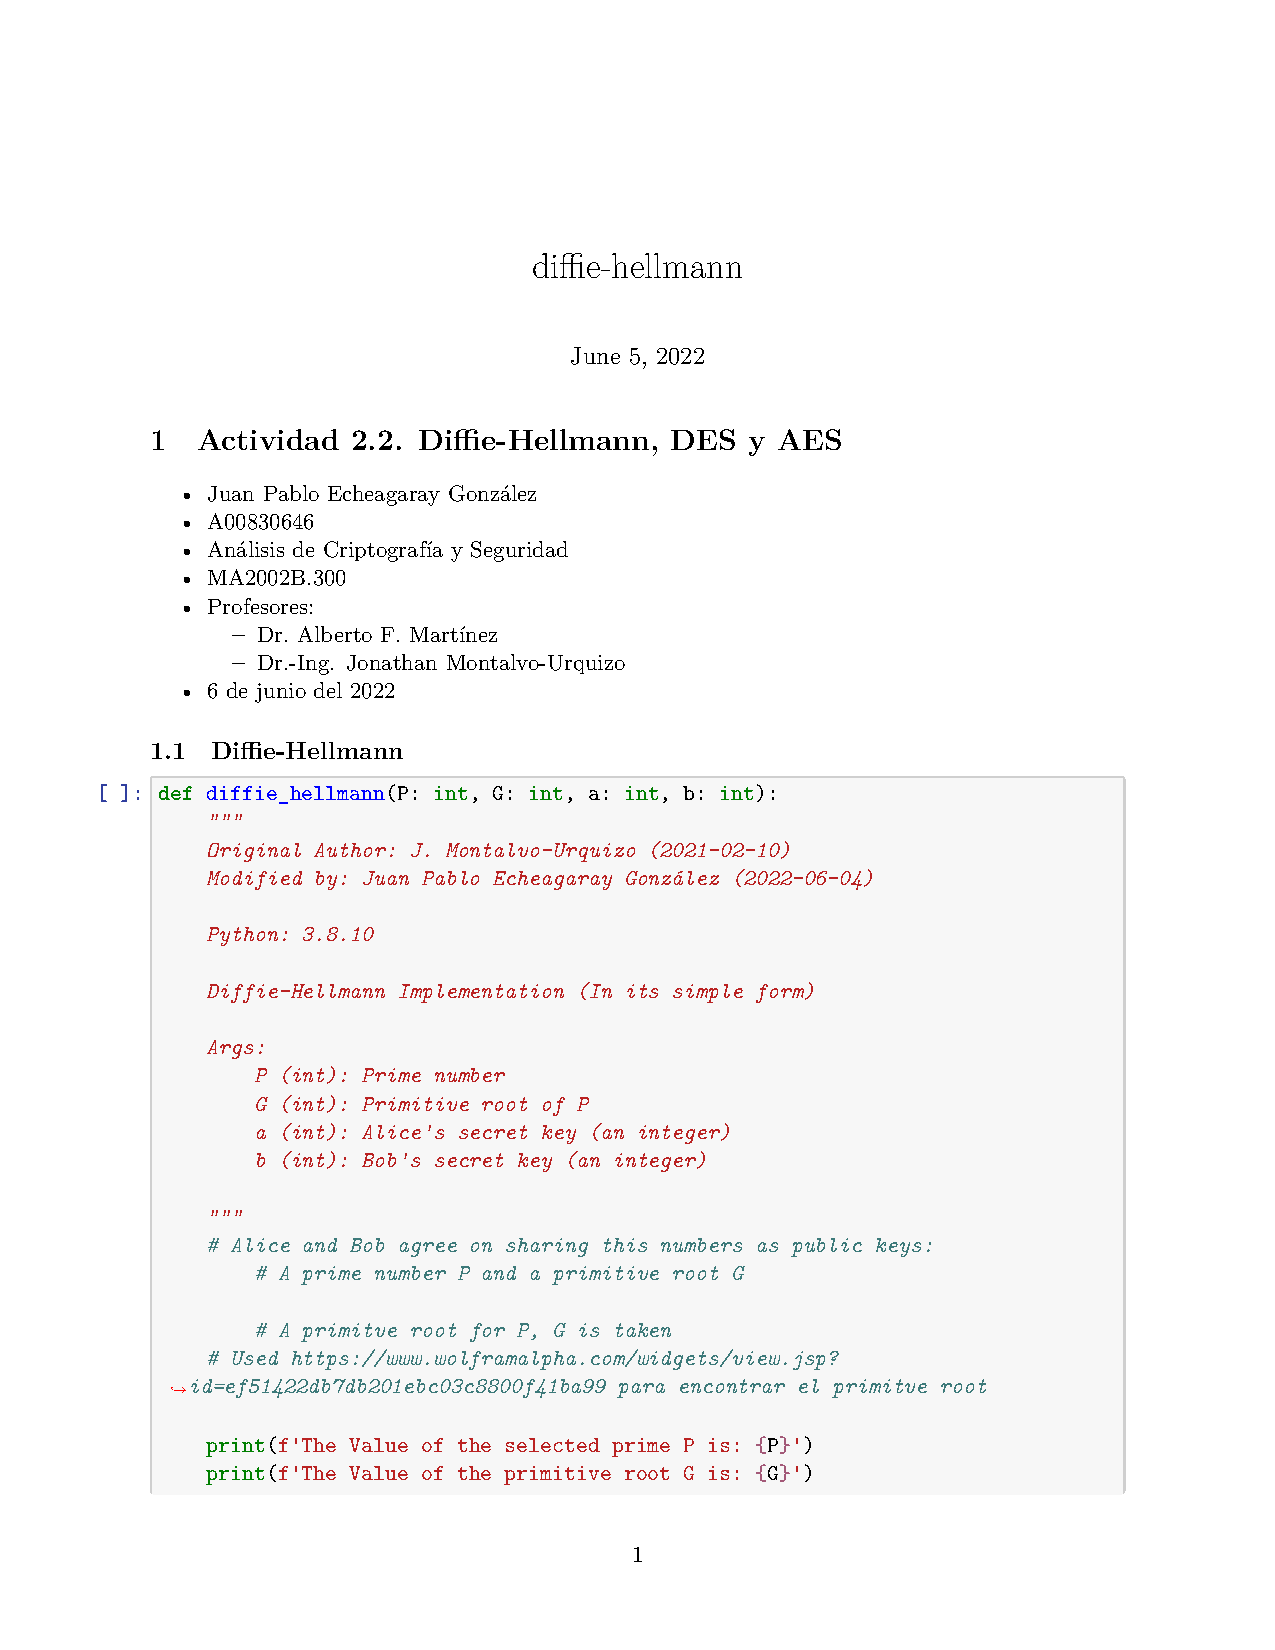
\includepdf[pages=-]{../diffie-hellmann.pdf}

    \section{Pruebas de AES en equipos distintos}

        \subsection{En Windows}

            \begin{figure}[!h]
                \centering
                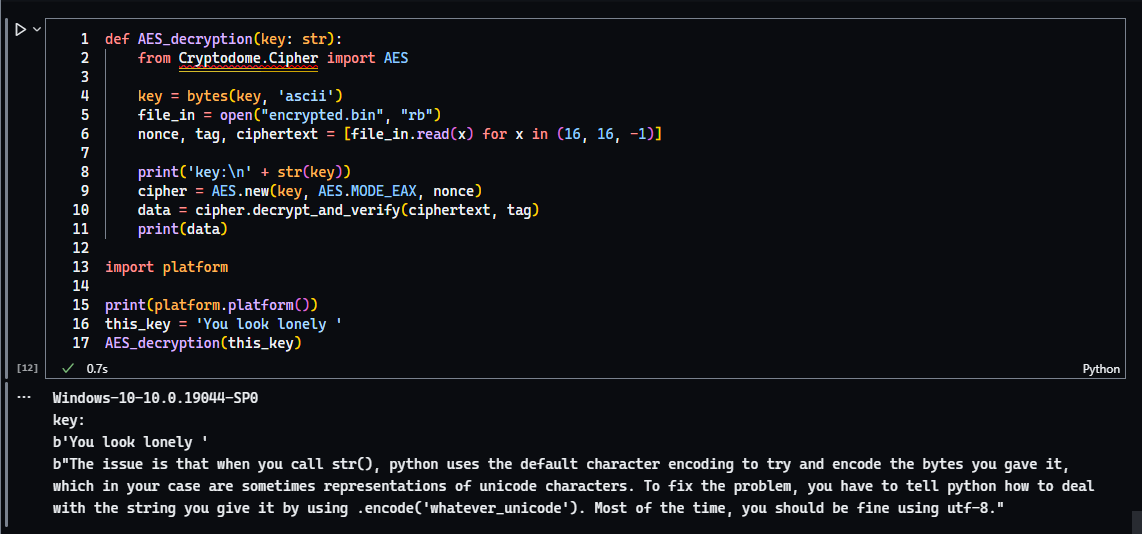
\includegraphics[scale=0.5]{img/windows-evidence.png}
                \caption{Evidencia de funcionamiento en máquina con Windows}
                \label{fig:windows}
            \end{figure}

        \subsection{En Google Colab}
        
            \begin{figure}[!h]
                \centering
                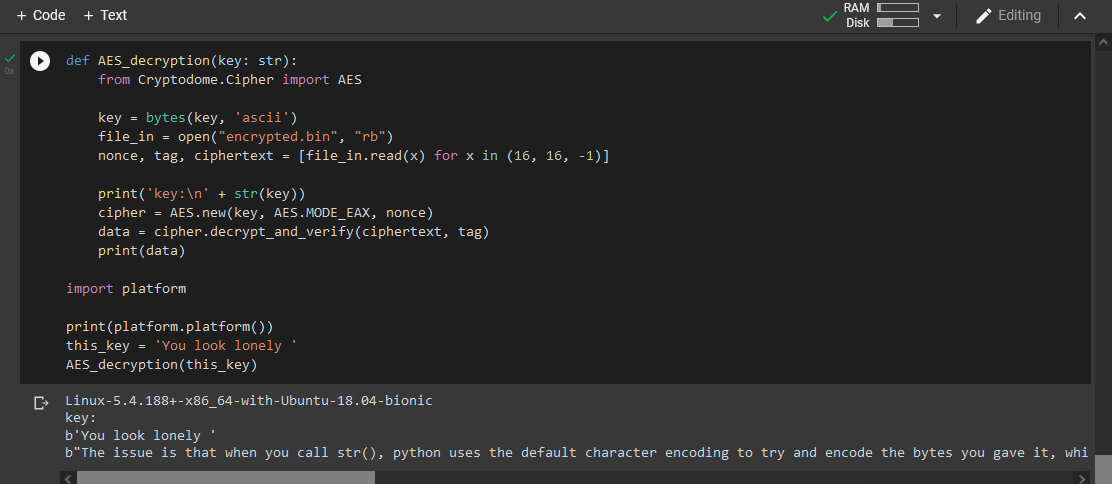
\includegraphics[scale=0.5]{img/colab-evidence.png}
                \caption{Evidencia de funcionamiento en máquina con máquina virtual en Google Colab}
                \label{fig:colab}
            \end{figure}
    
    \bibliographystyle{apalike}
    \bibliography{references.bib}
\end{document}